\documentclass[11pt]{article}
\usepackage[margin=1in]{geometry}
\usepackage[T1]{fontenc}
\usepackage{charter}
\usepackage{microtype}
\usepackage{amsmath}
\usepackage{graphicx}
\usepackage{booktabs}
\usepackage{tabularx}
\usepackage{caption}
\usepackage[hyphens]{url}
\emergencystretch=2em
\usepackage{xcolor}
\usepackage[authoryear,round]{natbib}
\usepackage[colorlinks=true,linkcolor={black},citecolor={blue!50!black},urlcolor={blue!50!black}]{hyperref}
\captionsetup{font=small,labelfont=bf}
\graphicspath{{../outputs/figures/}}
% generated by src/08_tex.py — do not edit by hand
\newcommand{\NCells}{15,160}
\newcommand{\NGridCells}{15,166}
\newcommand{\NCellYears}{300,471}
\newcommand{\NNbhd}{277}
\newcommand{\NScenes}{151}
\newcommand{\NScenesUsed}{111}
\newcommand{\NInventory}{193,009}
\newcommand{\NYoungA}{5,959}
\newcommand{\NYoungB}{12,612}
\newcommand{\NMid}{15,299}
\newcommand{\NMature}{50,542}
\newcommand{\NVacant}{44,469}
\newcommand{\EstA}{-0.026}
\newcommand{\LoA}{-0.047}
\newcommand{\HiA}{-0.005}
\newcommand{\EstB}{-0.015}
\newcommand{\LoB}{-0.031}
\newcommand{\HiB}{0.000}
\newcommand{\EstC}{-0.029}
\newcommand{\LoC}{-0.046}
\newcommand{\HiC}{-0.012}
\newcommand{\EstV}{0.013}
\newcommand{\LoV}{0.001}
\newcommand{\HiV}{0.024}
\newcommand{\EstAabs}{0.026}
\newcommand{\LoAabs}{0.005}
\newcommand{\HiAabs}{0.047}
\newcommand{\FiveTrees}{0.13}
\newcommand{\EstAtwentyfive}{-0.035}
\newcommand{\PreWald}{2.59}
\newcommand{\PreDf}{4}
\newcommand{\PreP}{0.63}
\newcommand{\EstStrict}{-0.027}
\newcommand{\LoStrict}{-0.048}
\newcommand{\HiStrict}{-0.006}
\newcommand{\EstYearFE}{-0.096}
\newcommand{\YearFERatio}{3.7}
\newcommand{\EstPlacebo}{-0.088}
\newcommand{\LoPlacebo}{-0.115}
\newcommand{\HiPlacebo}{-0.062}
\newcommand{\EstBin}{-0.089}
\newcommand{\LoBin}{-0.159}
\newcommand{\HiBin}{-0.019}
\newcommand{\NBinT}{4,741}
\newcommand{\NBinC}{6,064}
\newcommand{\EstLD}{-0.028}
\newcommand{\SeLD}{0.0072}
\newcommand{\RV}{3.1}
\newcommand{\RValpha}{1.5}
\newcommand{\PartialRtwo}{0.10}
\newcommand{\EstAdjThree}{-0.024}
\newcommand{\LoAdjThree}{-0.038}
\newcommand{\HiAdjThree}{-0.009}
\newcommand{\NCSA}{55}
\newcommand{\CSATrees}{30,792}
\newcommand{\CSAPreWald}{86}
\newcommand{\CSADoseMean}{210}
\newcommand{\CSALate}{-0.26}
\newcommand{\CSAPre}{-0.10}
\newcommand{\ScenesPerYearMin}{2}
\newcommand{\ScenesPerYearMax}{8}

\newcommand{\degC}{\,\textdegree C}

\title{\textbf{Do New Street Trees Cool the City?\\ Within-Neighborhood Evidence from Baltimore, 2006--2025}}
\author{Sahil\\[2pt]\small MSE in Data Science, Whiting School of Engineering, Johns Hopkins University, Baltimore, MD\\\small \texttt{sfnu1@jh.edu}}
\date{Working paper, October 2026}

\begin{document}
\maketitle

\begin{abstract}
\noindent Cities plant trees to adapt to extreme heat, but most evidence that trees cool cities compares places that already differ in many ways. We estimate what a municipal street-tree program actually delivered, using Baltimore's 2017--18 census of \NInventory{} public trees and planting sites and \NScenesUsed{} clear-sky Landsat summer scenes from 2006 to 2025. Trunk size dates young trees; empty sites the city judged plantable provide the comparison. On a grid of \NCells{} cells of 90\,m, an event-study design with cell and neighborhood-by-year fixed effects compares blocks within the same neighborhood in the same year. Each young street tree (trunk $\le$1.5\,in in 2017--18, planted roughly 2014--17) lowered its cell's summer surface temperature by \EstAabs\degC{} by 2022--25 relative to 2006--09 (95\% CI \LoAabs--\HiAabs). There was no detectable change before planting (joint pre-trend test $p=\PreP$), and the effect grew as the trees matured. The estimate is stable across weighting, clustering and data-quality choices. It is also robust to controlling every site type by year, and to an omitted confounder three times as strong as mature-tree density. Its size matches a simple shading calculation. A naive design comparing whole neighborhoods fails: neighborhoods that received more trees in 2013--20 were already cooling in 2009--12, before those plantings. Within-neighborhood comparison is therefore essential for evaluating urban greening. A placebo on sites judged unplantable also fails, which points to block-level changes such as demolitions that future work should measure directly.

\medskip\noindent\textbf{Keywords:} urban heat; street trees; program evaluation; event study; Landsat; surface temperature; Baltimore
\end{abstract}

\section{Introduction}

Planting trees is among the most popular heat-adaptation policies in American cities. Baltimore set a goal in 2007 of doubling its tree canopy from 20\% to 40\% by 2037 \citep{treebaltimore2018}, and its TreeBaltimore program and partners plant thousands of trees a year \citep{bnia}. The case for such programs rests mostly on a robust correlation: places with more canopy are cooler \citep{ziter2019}. That correlation does not answer the policy question a city faces, which is how much cooling \emph{new} plantings buy, and when.

Answering that question is hard for a reason familiar from program evaluation: plantings are not random. Cities target neighborhoods by need, residents request trees, and planting tends to coincide with other neighborhood change. Tree canopy itself carries a history of segregation and disinvestment \citep{locke2021,hoffman2020}. A comparison of planted and unplanted places mixes the effect of trees with the reasons those places were chosen. The closest causal evidence uses tree \emph{loss} from the emerald ash borer in Toronto \citep{han2024}. Evidence on tree \emph{gains} from an actual planting program is scarce.

This paper estimates the cooling effect of Baltimore's recent street-tree plantings with three design choices aimed at that selection problem. First, the comparison group is empty sites the city itself surveyed and judged plantable. Those sites passed the same streetscape screen as planted ones, but had no tree yet. Second, cell and neighborhood-by-year fixed effects compare 90\,m blocks only with other blocks in the same neighborhood in the same year. Third, trunk-size cohorts imply different planting windows, so each cohort predicts a different start date for cooling. That gives the design a built-in timing test.

We report four findings. (i) Young street trees cooled their blocks after, and only after, they were planted, with effects that grow over time. (ii) The magnitude, about \EstAabs\degC{} per tree in a 90\,m cell, is what simple shading arithmetic predicts. (iii) A design comparing whole neighborhoods fails its pre-trend test, showing how strongly neighborhood selection would bias naive estimates. (iv) A placebo on unplantable sites fails as well. We trace that failure to block-level trends in rowhouse neighborhoods and show that it does not move the main estimate.

\section{Setting and data}

\paragraph{Tree inventory.} Baltimore's Forestry Division conducted its first complete census of public street and park trees in 2017--18 \citep{baltimoretrees}. The public map service holds \NInventory{} records: live trees with species, trunk diameter at breast height (DBH) and condition, plus stumps and empty planting sites classified as plantable (``Vacant Site''), potential, or not suitable. Almost all records date from the census itself. The layer's planting-date field is filled for about 220 records, so the public data cannot date plantings directly. We therefore use trunk size: street trees are planted as nursery stock of roughly 1.5--2\,in caliper and add roughly 0.25--0.5\,in of diameter a year when young. A live street tree of DBH $\le$1.5\,in in 2017--18 was thus planted in roughly the preceding three years (``young-A'', \NYoungA{} trees). Trees of 1.5--3\,in were planted around 2010--15 (``young-B'', \NYoungB{}), and trees of 3--6\,in around 2003--11 (\NMid{}). These windows are approximate. Section~\ref{sec:results} tests them against the timing of cooling. The comparison group is the \NVacant{} plantable empty sites. We also count \NMature{} mature street trees (DBH $>$6\,in), stumps, dead trees and park trees.

\paragraph{Surface temperature.} We use Landsat Collection 2 Level-2 surface temperature for WRS-2 path 15, row 33, June--August 2006--2025, from Landsat~5, 7, 8 and 9 \citep{planetary}. Of \NScenes{} scenes with less than 60\% cloud cover, \NScenesUsed{} had at least 30\% of the city clear after masking cloud, cirrus, shadow, snow, water and fill pixels. Each year has between \ScenesPerYearMin{} and \ScenesPerYearMax{} usable scenes (Appendix Table~\ref{tab:scenes}). Surface temperature is $\mathrm{ST}\times0.00341802+149$\,K \citep{usgs2024}. Residual cloud pixels colder than the larger of 15\degC{} and the scene median minus 15\degC{} are dropped.

For each scene we subtract the city-wide median. This removes day-to-day weather and differences between sensors, leaving each pixel's temperature \emph{relative to the city that day}. Pixels are averaged into 90\,m cells, requiring at least four of nine valid. Each cell's relative temperatures are then averaged within a year. Landsat's thermal bands are natively 60--120\,m and delivered at 30\,m, so 90\,m cells are close to the sensors' true resolution. Of \NGridCells{} cells containing at least one inventory record, \NCells{} have usable temperature data; the analysis panel has \NCellYears{} cell-years in \NNbhd{} neighborhoods.

\paragraph{Neighborhood planting counts.} For a coarser second design we use TreeBaltimore's counts of trees planted per Community Statistical Area (CSA), 2013--2020: \CSATrees{} trees in \NCSA{} CSAs \citep{bnia}.

\section{Empirical strategy}

For cell $i$ in neighborhood $n(i)$ and year $t$, the main specification is
\begin{equation}
Y_{it} = \alpha_i + \delta_{n(i)t} + \sum_{k}\sum_{s\neq \mathrm{ref}} \beta_{ks}\, D_{ki}\, \mathbf{1}[t=s] + \sum_{c}\sum_{s\neq \mathrm{ref}} \gamma_{cs}\, X_{ci}\, \mathbf{1}[t=s] + \varepsilon_{it},
\label{eq:es}
\end{equation}
where $Y_{it}$ is the cell's mean relative surface temperature (\degC). $D_{ki}$ counts trees of cohort $k\in\{$young-A, young-B, 3--6\,in$\}$, and $X_{ci}$ counts plantable empty sites, mature trees and stumps. The reference period pools 2006--09. Counts are capped at 10 per cell (about the 99th percentile). Observations are weighted by the number of clear scenes, and standard errors are clustered by neighborhood (\NNbhd{} clusters). Estimation uses \texttt{pyfixest} \citep{pyfixest}.

Each $\beta_{ks}$ measures how much a cell's temperature changed in year $s$, relative to 2006--09, for each additional tree of cohort $k$. The comparison is with cells in the same neighborhood and year that hold the same mix of other sites. The neighborhood-by-year effects $\delta_{n(i)t}$ absorb anything that moves a whole neighborhood in a given year, such as redevelopment waves, citywide programs or targeting of planting by neighborhood. Because treatment timing is inferred rather than observed, we do not use staggered-adoption estimators \citep{callaway2021,sun2021}. Instead we read each cohort's coefficient path against its implied planting window. Identification requires that, within a neighborhood, blocks that received more young trees would otherwise have followed the same temperature path as blocks with more empty plantable sites. Pre-period coefficients test this, with the usual caution that passing a pre-test is not proof \citep{roth2022}.

\section{Results}\label{sec:results}

\subsection{Main estimates}

Figure~\ref{fig:es} and Table~\ref{tab:main} show the results. For the youngest cohort (planted around 2014--17), coefficients stay near zero through 2017. A joint test of the 2010--13 coefficients does not reject zero ($\chi^2=\PreWald$, $\mathit{df}=\PreDf$, $p=\PreP$). Cooling appears from 2018 and deepens to $\EstAtwentyfive$\degC{} per tree in 2025. Pooled over 2022--25, each young tree lowered its cell's relative surface temperature by \EstAabs\degC{} (coefficient $\EstA$, 95\% CI $\LoA$ to $\HiA$). A cell with five such trees, an ordinary planted block face, was about \FiveTrees\degC{} cooler than it would otherwise have been.

The 3--6\,in cohort, planted around 2003--11, shows cooling from about 2016 that reaches $\EstC$\degC{} per tree in 2022--25 ($\LoC$ to $\HiC$). That fits trees whose crowns began to shade meaningfully in the mid-2010s. The 1.5--3\,in cohort shows a smaller late effect ($\EstB$, CI $\LoB$ to $\HiB$) and a small dip in 2010--12 that does not fit its implied window cleanly. We report it as is. Plantable empty sites warm slightly relative to the base period ($\EstV$\degC{} per site in 2022--25). That is consistent with some of them being trees lost between 2006 and the 2017--18 census.

A binary version gives the same answer. It compares the \NBinT{} cells with at least one young tree to the \NBinC{} cells with plantable empty sites but no young trees. The 2022--25 effect is $\EstBin$\degC{} per cell (95\% CI $\LoBin$ to $\HiBin$).

\begin{figure}[t]\centering
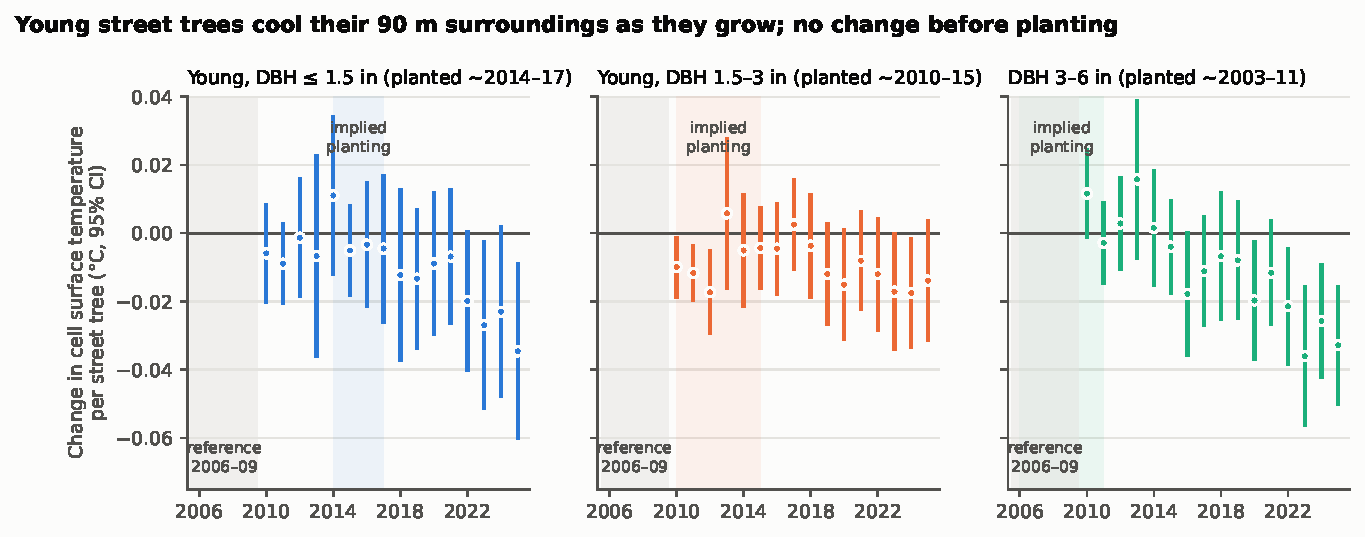
\includegraphics[width=\textwidth]{fig1_event_study_cohorts.pdf}
\caption{Change in 90\,m cell summer surface temperature per street tree, by trunk-size cohort, relative to 2006--09. Points are year-specific coefficients $\beta_{ks}$ from equation~\eqref{eq:es} with 95\% confidence intervals (standard errors clustered by neighborhood). Shaded bands mark the reference period (grey) and each cohort's approximate planting window implied by trunk size (colour).}
\label{fig:es}
\end{figure}

\begin{table}[t]\centering\small
\caption{Change in cell surface temperature per tree or site (\degC), relative to 2006--09, pooled by period. Clustered standard errors in parentheses; $^{*}$ 95\% CI excludes zero. All coefficients come from one regression (equation~\ref{eq:es}).}\label{tab:main}
\begin{tabular}{@{}lcccc@{}}\toprule
 & 2010--13 & 2014--17 & 2018--21 & 2022--25 \\\midrule
Young, DBH $\le$ 1.5 in & $-0.006$ {\footnotesize $(0.007)$} & $0.000$ {\footnotesize $(0.008)$} & $-0.010$ {\footnotesize $(0.009)$} & $-0.026^{*}$ {\footnotesize $(0.011)$} \\
Young, DBH 1.5--3 in & $-0.008$ {\footnotesize $(0.005)$} & $-0.003$ {\footnotesize $(0.006)$} & $-0.010$ {\footnotesize $(0.007)$} & $-0.015$ {\footnotesize $(0.008)$} \\
DBH 3--6 in & $0.007$ {\footnotesize $(0.006)$} & $-0.008$ {\footnotesize $(0.007)$} & $-0.012$ {\footnotesize $(0.008)$} & $-0.029^{*}$ {\footnotesize $(0.008)$} \\
Vacant plantable site & $0.004$ {\footnotesize $(0.003)$} & $0.012^{*}$ {\footnotesize $(0.004)$} & $0.010^{*}$ {\footnotesize $(0.005)$} & $0.013^{*}$ {\footnotesize $(0.006)$} \\

\bottomrule\end{tabular}
\end{table}

\subsection{Is the magnitude plausible?}

A useful check is whether the estimate is physically reasonable. A street tree a decade after planting has a crown perhaps 3--5\,m across, about 7--20\,m$^2$, or roughly 0.1--0.25\% of a 90\,m cell (8,100\,m$^2$). If shaded surfaces at Landsat's late-morning overpass are roughly 10--15\degC{} cooler than sunlit pavement, a tree should lower the cell average by roughly 0.01--0.04\degC. These are assumed round numbers, not measurements, but the estimated \EstAabs\degC{} falls inside this range. The effect is small per tree because a single young tree shades a small area. It is not small relative to what the tree physically covers.

\subsection{Robustness}

Table~\ref{tab:robust} re-estimates the pooled 2022--25 effect under alternative choices. The young-tree estimate ranges from $-0.023$ to $-0.028$\degC{} across specifications that drop weights, cluster by \NCSA{} CSAs, keep only cell-years with at least three clear scenes, or drop cells with park trees. The most demanding specification adds plantable, potential and not-suitable sites, stumps and dead trees, each interacted with year. That absorbs differential trends by block type, and the estimate is $\EstStrict$\degC{} ($\LoStrict$ to $\HiStrict$).

Dropping the neighborhood-by-year effects in favour of plain year effects inflates the estimate to $\EstYearFE$\degC{}, \YearFERatio{} times larger. Neighborhood-wide trends are large, and they are correlated with where trees were planted.

\begin{table}[t]\centering\small
\caption{Robustness of the 2022--25 effect per tree (\degC), relative to 2006--09, by cohort. 95\% confidence intervals in brackets.}\label{tab:robust}
\begin{tabularx}{\textwidth}{@{}Xccc@{}}\toprule
Specification & DBH $\le$1.5\,in & 1.5--3\,in & 3--6\,in \\\midrule
Main specification & $-0.026$ {\footnotesize $[-0.047, -0.005]$} & $-0.015$ {\footnotesize $[-0.030, 0.000]$} & $-0.029$ {\footnotesize $[-0.046, -0.012]$} \\
All site types $\times$ year (strictest controls) & $-0.027$ {\footnotesize $[-0.048, -0.006]$} & $-0.021$ {\footnotesize $[-0.037, -0.005]$} & $-0.032$ {\footnotesize $[-0.048, -0.015]$} \\
No site-type controls & $-0.026$ {\footnotesize $[-0.047, -0.005]$} & $-0.015$ {\footnotesize $[-0.030, 0.001]$} & $-0.031$ {\footnotesize $[-0.047, -0.014]$} \\
Unweighted & $-0.028$ {\footnotesize $[-0.048, -0.007]$} & $-0.015$ {\footnotesize $[-0.031, 0.000]$} & $-0.030$ {\footnotesize $[-0.046, -0.014]$} \\
Clustered by 55 CSAs & $-0.026$ {\footnotesize $[-0.047, -0.006]$} & $-0.015$ {\footnotesize $[-0.028, -0.002]$} & $-0.029$ {\footnotesize $[-0.042, -0.016]$} \\
Cell-years with $\ge$3 clear scenes & $-0.026$ {\footnotesize $[-0.047, -0.005]$} & $-0.015$ {\footnotesize $[-0.030, 0.000]$} & $-0.029$ {\footnotesize $[-0.046, -0.013]$} \\
Excluding cells with park trees & $-0.023$ {\footnotesize $[-0.045, -0.002]$} & $-0.014$ {\footnotesize $[-0.030, 0.002]$} & $-0.024$ {\footnotesize $[-0.040, -0.008]$} \\
Year FE only (no neighborhood $\times$ year FE) & $-0.096$ {\footnotesize $[-0.131, -0.060]$} & $-0.078$ {\footnotesize $[-0.102, -0.055]$} & $-0.073$ {\footnotesize $[-0.101, -0.045]$} \\

\bottomrule\end{tabularx}
\end{table}

\subsection{Sensitivity to unobserved confounding}

To ask how strong an unmeasured confounder would need to be, we follow \citet{cinelli2020} on a long-difference version of the model. The outcome is each cell's change in mean relative temperature from 2006--09 to 2022--25. It is regressed on the tree and site counts with neighborhood fixed effects, which gives $\EstLD$\degC{} per young tree (SE \SeLD). The treatment's partial $R^2$ is \PartialRtwo\%. The robustness value is \RV\%: a confounder would have to explain at least \RV\% of the residual variance of both young-tree counts and temperature change to remove the estimate (\RValpha\% to make it insignificant at the 5\% level).

Table~\ref{tab:sens} benchmarks this against an observed covariate, mature-tree density. A confounder even three times as strong would move the estimate only to $\EstAdjThree$\degC{} (95\% CI $\LoAdjThree$ to $\HiAdjThree$).

\begin{table}[t]\centering\small
\caption{Bounds on the long-difference estimate per young tree under a hypothetical confounder as strong as $k$ times mature-tree density \citep{cinelli2020}. Partial $R^2$ in percent.}\label{tab:sens}
\begin{tabular}{@{}lcccc@{}}\toprule
Confounder strength & $R^2_{D\sim Z|X}$ & $R^2_{Y\sim Z|D,X}$ & Adjusted estimate & 95\% CI \\\midrule
1$\times$ mature-tree density & 0.16 & 0.13 & $-0.026$ & $[-0.040, -0.012]$ \\
2$\times$ mature-tree density & 0.32 & 0.27 & $-0.025$ & $[-0.039, -0.011]$ \\
3$\times$ mature-tree density & 0.48 & 0.40 & $-0.024$ & $[-0.038, -0.009]$ \\

\bottomrule\end{tabular}
\end{table}

\subsection{Why within-neighborhood comparison matters}

Figure~\ref{fig:design} contrasts the main design with a coarser one: CSA-level relative temperature regressed on trees planted per km$^2$ in 2013--20, interacted with year, with CSA and year fixed effects. Here the pre-planting years already show cooling. The 2009--12 coefficients average $\CSAPre$\degC{} per 100 trees/km$^2$ and are jointly far from zero ($\chi^2=\CSAPreWald$, $p<0.001$). Neighborhoods that later received more trees were already cooling for other reasons. A naive reading of the later coefficients (about $\CSALate$\degC{} per 100 trees/km$^2$) would credit trees with that trend. Within-neighborhood comparison removes it, and the block-level pre-trend test passes.

\begin{figure}[t]\centering
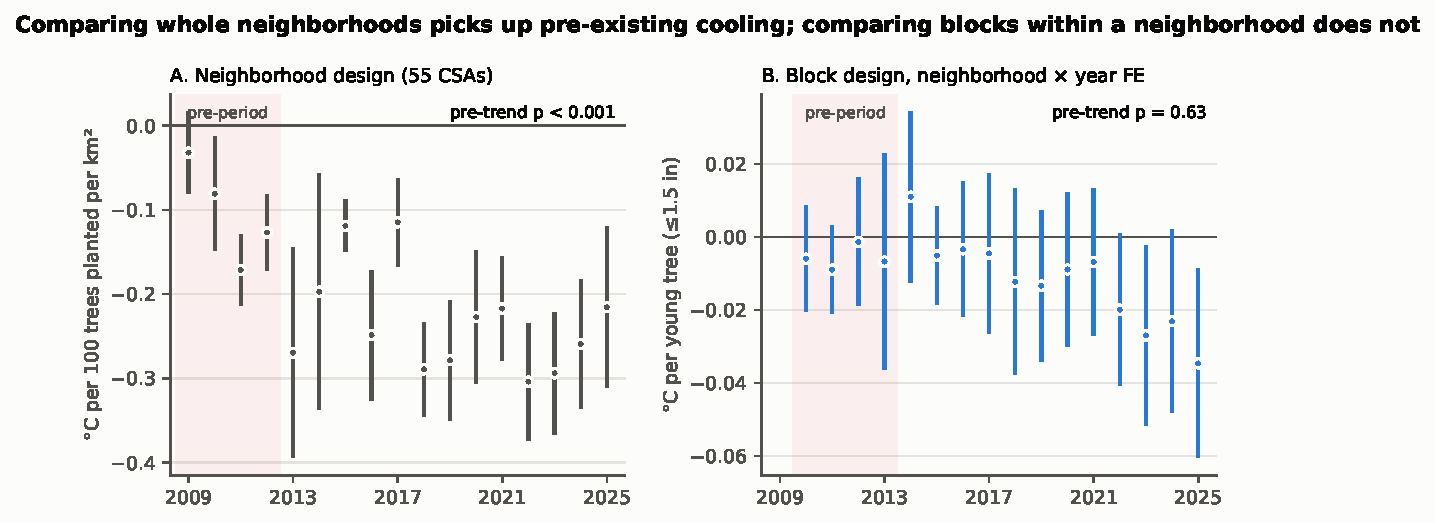
\includegraphics[width=\textwidth]{fig2_design_comparison.pdf}
\caption{(A) Neighborhood design: \NCSA{} Community Statistical Areas, dose = hundreds of trees planted per km$^2$ in 2013--20 \citep{bnia}, reference 2006--08. (B) Block design: young-tree (DBH $\le$1.5\,in) coefficients from equation~\eqref{eq:es}. Shaded: years before planting in each design.}
\label{fig:design}
\end{figure}

\subsection{A failed placebo}

As a placebo we estimated the same model for empty sites the foresters judged \emph{not suitable} for planting. They should show no systematic temperature change. They do: $\EstPlacebo$\degC{} per site by 2022--25 (95\% CI $\LoPlacebo$ to $\HiPlacebo$), with cooling that begins around 2010. These sites concentrate in dense rowhouse neighborhoods with heavy vacancy (among them Harlem Park, Sandtown-Winchester, Upton, Broadway East and Oliver). In such neighborhoods, demolition of vacant houses and greening of the resulting lots can lower surface temperature independently of street trees; greening programs of this kind are a policy in their own right \citep{branas2018}. The failure shows that block types follow different temperature paths within a neighborhood. Controlling for every site type by year absorbs this and leaves the young-tree estimate essentially unchanged (Table~\ref{tab:robust}). Even so, demolition and lot-greening records should be added as direct, time-varying controls.

\section{Discussion}

Three limitations bound these results. First, planting dates are inferred from trunk size, so treatment timing is fuzzy. The cohort windows are approximate, and the clean timing in the youngest cohort is more convincing than the mixed pattern in the 1.5--3\,in cohort. Work-order records with exact dates would allow a staggered-adoption estimator \citep{callaway2021}. Second, only trees alive at the 2017--18 census are counted. Trees that died before the census are not, so the estimates describe surviving plantings. A program-level estimate would net out mortality. Third, the outcome is daytime surface temperature on clear summer days. It is a good measure of shading but overstates what residents feel in the air at night, when heat-health risk is high.

Within those limits, the results support two conclusions. For Baltimore, recent street trees have begun to cool their blocks, and the effect is still growing as they mature. The 40\% canopy goal implies benefits that arrive with a lag of several years after planting. For evaluating urban greening anywhere, the contrast between Figure~\ref{fig:design}A and~B is the main methodological lesson. Neighborhood-level comparisons inherit the targeting of programs and the larger changes under way in the places they target. Comparisons within neighborhoods, against sites that passed the same eligibility screen, can separate the two.

\section{Conclusion}

Using Baltimore's own census of street trees and empty planting sites with two decades of Landsat imagery, we find that young street trees lowered the summer surface temperature of their 90\,m surroundings by about \EstAabs\degC{} each. The cooling began only after planting, grew with tree age, and survives a range of robustness and sensitivity checks. The next steps are to obtain dated planting records, add demolition and lot-greening controls, examine heterogeneity by historical redlining and baseline canopy, and test the result against air-temperature measurements.

\paragraph{Data and code availability.} All inputs are public. The extraction script, packed dataset (SHA-256 recorded), analysis code, tables and figures are in the project repository \texttt{baltimore\_tree\_cooling}. One command (\texttt{bash run\_all.sh}) rebuilds every number in this paper. The numbers are written to \texttt{macros.tex} automatically.

\bibliographystyle{plainnat}
\bibliography{refs}

\appendix
\section{Landsat scenes used}

\begin{table}[ht]\centering\small
\caption{Clear-sky summer scenes used, by year and satellite (L5--L9 = Landsat 5--9).}\label{tab:scenes}
\begin{tabular}{@{}lccccc|lccccc@{}}\toprule
Year & L5 & L7 & L8 & L9 & Total & Year & L5 & L7 & L8 & L9 & Total \\\midrule
2006 & 4 & 4 & 0 & 0 & 8 & 2016 & 0 & 2 & 3 & 0 & 5 \\
2007 & 4 & 4 & 0 & 0 & 8 & 2017 & 0 & 2 & 1 & 0 & 3 \\
2008 & 2 & 4 & 0 & 0 & 6 & 2018 & 0 & 3 & 1 & 0 & 4 \\
2009 & 3 & 2 & 0 & 0 & 5 & 2019 & 0 & 4 & 2 & 0 & 6 \\
2010 & 3 & 4 & 0 & 0 & 7 & 2020 & 0 & 2 & 4 & 0 & 6 \\
2011 & 4 & 2 & 0 & 0 & 6 & 2021 & 0 & 3 & 3 & 0 & 6 \\
2012 & 0 & 3 & 0 & 0 & 3 & 2022 & 0 & 1 & 2 & 3 & 6 \\
2013 & 0 & 1 & 1 & 0 & 2 & 2023 & 0 & 1 & 2 & 3 & 6 \\
2014 & 0 & 2 & 1 & 0 & 3 & 2024 & 0 & 0 & 3 & 3 & 6 \\
2015 & 0 & 4 & 4 & 0 & 8 & 2025 & 0 & 0 & 4 & 3 & 7 \\

\bottomrule\end{tabular}
\end{table}

\end{document}
